\section{Our Solution: $\vats$}\label{sec:sol}
In this part, we address the second technical challenge: \emph{how to devise an efficient sampling algorithm that provides guaranteed visual fidelity?}
Specifically, we first propose a visual fidelity-guaranteed sampling algorithm $\vats$ in Section~\ref{sec:greedy}. Next, we devise optimizations to improve the efficiency of $\vats$ in Section~\ref{sec:opt}.

\subsection{Visual Fidelity-Guaranteed Sampling}\label{sec:greedy}
%Due to the hardness of Problem~\ref{prob:def}, the straight-forward solution is uniform random sampling $\rand$.
%This solution randomly selects $k$ trajectories from the dataset $\D$ and stores them in the result set $\oR$. The selected trajectories in $\oR$ are rendered as the visualization result.
%Obviously, uniform random sampling $\rand$ does not provide any guarantee on the visual fidelity of the sampled set.

Our visual fidelity-guaranteed sampling method $\vats$ is presented in Algorithm~\ref{alg:greedy}, which employs a greedy paradigm.
In particular, it finds the trajectory $tmp$ in $\D$ that maximizes $| tmp \cup \oR|$ at each iteration, as shown in Line~\ref{line:max} of Algorithm~\ref{alg:greedy}.
It terminates after $k=\alpha |\D|$ iterations and returns $\oR$ as the result set for rendering.

%\vspace{-2mm}
\begin{algorithm}
    \caption{$\vats(\D,k=\alpha |\D|)$} \label{alg:greedy}
    \begin{algorithmic}[1]
    \State Initialize result set $\oR \leftarrow \emptyset$
    \While{$|\oR| < k$}
        \State $tmp \leftarrow argmax_{t_i \in \D} |t_i \cup \oR|$ \label{line:max}
        \State $\oR \leftarrow \oR \cup \{ tmp \}$
    \EndWhile
    \State Return $\oR$
    \end{algorithmic}
\end{algorithm}


Interestingly, Algorithm~\ref{alg:greedy} provides provable visual fidelity guarantee for the returned result $\oR$, as stated in Theorem~\ref{the:ratio}.
%~\footnote{We omitted all the proofs of the theorems and lemmata in this work due to space reasons, and refer the interested readers to our technical report\cite{techreport}.}

\begin{theorem}~\label{the:ratio}
Define the visual fidelity of a sample set $\mathcal{S}$ as $f(\mathcal{S})=1-loss(\V(\D),\V(\mathcal{S}))$. Let the sized-k result produced by Algorithm~\ref{alg:greedy} be $\mathcal{R}$ and the sized-k solution of Equation~\eqref{eq:opp} be $\mathcal{R}^{\star}$, we have $f(\mathcal{R})\ge 0.632*f(\mathcal{R}^{\star})$.
\end{theorem}

Theorem~\ref{the:ratio} follows directly from the submodularity of the visual fidelity function $f(\mathcal{S})$ as it is well known that the greedy solution provides a $0.632$ approximation of the optimal solution for a submodular function. We show that submodularity of $f(\mathcal{S})$ as follows.      

\begin{lemma}[Submodularity]\label{lem:submodular}
	Define the contribution of a trajectory $t$ to the result set $\oR$ as $\Delta(\oR, t) = |V(\oR \cup t)| - |V(\oR)|$.
	Given a trajectory $t$ and two result sets $\oR,\oR^{'}$, if $\oR \subset \oR^{'}$, then $ \Delta(\oR, t) \geq \Delta(\oR^{'}, t)$.
\end{lemma}


%\REPORT{
\begin{proof}
	The contribution value of trajectory $t$ w.r.t. a given result set $\oR$ (i.e., $\Delta(\oR, t) = |V(\oR \cup t)| - |V(\oR)|$) is the newly covered pixels, which can be expressed as $|V(t)| - |V(\oR \cap t)|$.
	We have $t \cap \oR \subseteq  t \cap \oR^{'}$ as $\oR^{'}$ is a superset of $\oR$, which implies $|V(t)| - |V(t \cap \oR)| \geq |V(t)| - |V(t \cap \oR^{'})|$.
	Thus, it holds that $\Delta(\oR, t) = |V(\oR \cup t)| - |V(\oR)| \geq |V(\oR^{'} \cup t)| - |V(\oR^{'})|= \Delta(\oR^{'}, t)$.
\end{proof}
%}


%\begin{proof}
%The optimal solution of Problem~\ref{prob:def} covers $f(\mathcal{R}^{\star})$ pixels in $k$ iterations.
%Let $a_i$ be the number of newly covered pixels at the $i$-th iteration, $b_i$ is the total number of covered pixels up to the $i$-th iteration (i.e., $b_i = \sum_{j=1}^{i}a_i$),
%and $c_i$ be the uncovered pixels after $i$-th iteration (i.e., $c_i = f(\mathcal{R}^{\star})-b_i$).
%According to greedy paradigm, we can conclude the number of newly covered pixels at the $(i+1)$-th iteration is always greater than or equal to $\frac{1}{k}$ of the number of uncovered pixels after the $i$-th iteration, i.e., $a_{i+1} \geq \frac{c_i}{k}$.
%We prove Theorem~\ref{the:ratio} by proving $c_{i+1} \leq (1-1/k)^{i+1} \cdot f(\mathcal{R}^{\star})$.
%It holds $c_1 \leq (1-1/k) \cdot f(\mathcal{R}^{\star})$ as follows.
%\begin{align} \nonumber
%& a_1 \geq c_0 \cdot 1/k = 1/k \cdot f(\mathcal{R}^{\star}) \text{~~~as we concluded~~~} a_{i+1} \geq \frac{c_i}{k}\\ \nonumber
% \Leftrightarrow  & b_1 \geq 1/k \cdot f(\mathcal{R}^{\star})  \Leftrightarrow  -b_1 \leq - 1/k \cdot f(\mathcal{R}^{\star})  \text{~~~as~~~} a_1 = b_1\\ \nonumber
% \Leftrightarrow & f(\mathcal{R}^{\star}) - b_ 1 \leq f(\mathcal{R}^{\star}) - 1/k \cdot f(\mathcal{R}^{\star})  \Leftrightarrow  c_1 \leq (1-1/k) \cdot f(\mathcal{R}^{\star})
%\end{align}
%For inductive hypothesis assume $c_{i} \leq (1-1/k)^i \cdot f(\mathcal{R}^{\star})$. Thus,
%\begin{align} \nonumber
%& c_{i+1} = c_i - a_{i+1} \leq c_i - c_i/k = (1-1/k) \cdot c_i =  (1-1/k)^{i+1} \cdot f(\mathcal{R}^{\star})
%\end{align}
%
%Hence, it holds $c_k \leq (1-1/k)^{k} \cdot f(\mathcal{R}^{\star})$.
%It is equivalent to $b_k = f(\mathcal{R}) \geq (1 - (1-1/k)^{k}) \cdot f(\mathcal{R}^{\star}) \geq (1-1/e) \cdot f(\mathcal{R}^{\star}) \approx 0.632 \cdot f(\mathcal{R}^{\star})$.
%\end{proof}

Although Algorithm~\ref{alg:greedy} provides fidelity guarantee for the result set $\oR$, it has a high time complexity, which we show in the following analysis.  

 


%With the above theoretical analysis, Algorithm~\ref{alg:greedy} offers a visual fidelity-guaranteed sampling algorithm for the large-scale trajectory data visualization problem.
%However, as the time complexity analyzed in Lemma~\ref{lem:cost}, it is not scalable to large-scale trajectory datasets (e.g., millions of trajectories).


\begin{lemma}[Time Complexity]~\label{lem:cost}
	Given trajectory dataset $\D$ and an integer $k = \alpha |\D|$, the time complexity of Algorithm~\ref{alg:greedy} is $O(\alpha \cdot m \cdot |\D|^2)$, where $m$ is the maximum length of all trajectories in dataset $\D$.
\end{lemma}


\begin{proof}
	In each iteration,
	Algorithm~\ref{alg:greedy} computes the uncovered pixels of each trajectory in dataset $\D$ with $O(m)$ cost.
	As the dataset $\D$ has $O(|\D|)$ trajectories and Algorithm~\ref{alg:greedy} runs for $k = \alpha |\D|$ iterations, the total cost is $O(k \cdot m \cdot |\D|)=O(\alpha \cdot m \cdot |\D|^2)$.
\end{proof}


The high complexity of Algorithm~\ref{alg:greedy} hurts its scalability for large-scale trajectory datasets. For example, the \pt{} dataset contains 2.39 millions taxi trajectories, and the longest trajectory has 3,490 GPS points.
It takes 413.6 seconds for Algorithm~\ref{alg:greedy} to obtain a result set $\oR$ with sampling rate $0.1\%$.    Obviously, the running time is too long for interactive trajectory exploration.

\subsection{Heap-based Lazy Computation}\label{sec:opt}




\begin{figure}
	\centering
	\small
	\begin{tabular}{cc}
		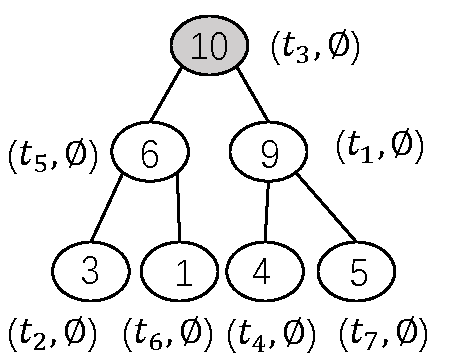
\includegraphics[width=0.35\columnwidth]{pictures/1st}
		&
		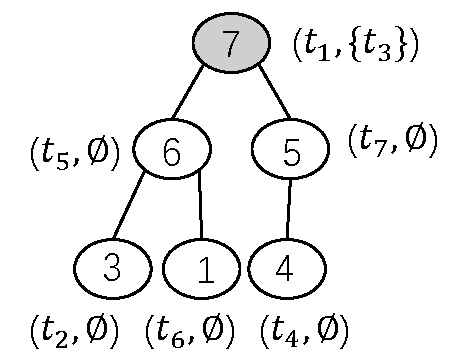
\includegraphics[width=0.35\columnwidth]{pictures/2nd}
		\\
		(A) 1st iteration
		&
		(B) 2nd iteration
	\end{tabular}
	\caption{Lazy computing manner.} \label{fig:heap} %via the submodularity in Lemma~\ref{lem:submodular}
\end{figure}







Algorithm~\ref{alg:greedy} essentially adds the trajectory that maximizes $\Delta(\oR, t) = |V(\oR \cup t)| - |V(\oR)|$ to $\oR$ in each iteration. Lemma~\ref{lem:submodular} shows that the contribution of a trajectory (i.e., $\Delta(\oR, t)$) cannot increase when Algorithm~\ref{alg:greedy} runs for more iterations because $ \Delta(\oR^{'}, t) \le \Delta(\oR, t) $ for  $\oR \subset \oR^{'}$. Based on this property, we can use  $\Delta(\oR, t)$ calculated in the previous iterations to prune a trajectory $t$ from computation. If we have $\Delta(\oR, t)\le \Delta(\oR^{'}, t')$, in which $\oR$ and $\oR^{'}$ are a previous and the current sample set, respectively, we know that $t$ can not be added to the sample set in the current iteration.         

 

To implement this idea, we maintain a max-heap for the number of uncovered pixels of each trajectory and update the max-heap in a lazy fashion. 
That is, the contribution of a trajectory is computed only when necessary.
Figure~\ref{fig:heap}(a) shows a tiny max-heap example for the numbers of uncovered pixels of trajectories from $t_1$ to $t_7$ with result set $\oR=\emptyset$.
At the first iteration, the root node of the max-heap, $t_3$ in Figure~\ref{fig:heap}(A), is selected.
At the second iteration, the number of uncovered pixels of the root node $t_1$ is updated to 7 w.r.t. result set $\oR = \{t_3 \}$ (see the gray node in Figure~\ref{fig:heap}(B)).
Then $t_1$ is selected at the second iteration without computing the number of uncovered pixels for other trajectories, i.e., all white nodes in Figure~\ref{fig:heap}(B).
The reason is that the contributions of these trajectories are all less than 7 according to the submodularity in Lemma~\ref{lem:submodular}.

%In summary, the number of uncovered pixels in each trajectory will only be computed with the latest result set $\oR$ when it is necessary in the lazy computing manner,
%e.g., only $t_1$ will be updated at the 2nd iteration in Figure~\ref{fig:heap}.
%It reduces many unnecessary computations through the lazy updating manner, e.g., all white nodes did not update at the 2nd iteration in the above example.

%We then analyze the time complexity of Algorithm~\ref{alg:greedy} with lazy computing manner in Theorem~\ref{lem:lazy}.
%
%\begin{lemma}[Optimized Time Complexity]~\label{lem:lazy}
%Given trajectory dataset $\D$ and an integer $k= \alpha |\D|$, the time complexity of Algorithm~\ref{alg:greedy} with lazy computing manner is $O(\alpha \cdot m \cdot x |\D| \log |\D|)$, where $x$ is the number of contribution computations among all $k$ iterations and $x \ll |\D|$.
%\end{lemma}
%
%\begin{proof}
%It first takes $O(|\D|)$ time to construct the max-heap~\cite{cormen2009introduction}.
%It incurs $O( m \cdot x \log |\D|)$ cost to select the trajectory with maximum uncovered pixels at each iteration ($k$ iterations in total).
%Hence, the overall cost is $O(|\D| + k \cdot m \cdot t \log |\D|)$.
%\end{proof}


The efficiency of Algorithm~\ref{alg:greedy} is significantly improved with heap-based lazy computation.
To exemplify, Algorithm~\ref{alg:greedy} takes 413.6 seconds to return the results with sampling rate $0.1\%$ on the \pt{} taxi trajectory dataset. In contrast, our performance-optimized $\vats$ needs only 1.2 seconds.


\section{Advanced Approach: $\avats$}\label{sec:aa}

In the previous section, we presented the $\vats$ algorithm, which produces fidelity-guaranteed samples and runs efficiently. 
In this section, we focus on the third technical challenge: \emph{how to tackle the visual clutter problem in large trajectory visualization}?
In particular, we devise an advanced approach $\avats$ by considering
(i) trajectory data distribution, and (ii) human perception capability.
We elaborate (i) and (ii) by the examples in Figure~\ref{fig:delta}.


\stitle{Trajectory data distribution} Considering the \pt{} trajectory dataset, Figure~\ref{fig:delta}(A) is the visualization result of $\vats$ with sampling ratio $0.5\%$. It is obvious that the trajectories follow a non-uniform distribution, and there are some dense regions and sparse regions as illustrated by the rectangles in Figure~\ref{fig:delta}(A).

      
%Obviously, the real-world trajectory dataset is non-uniform distributed.
%For example, the trajectories in dense region are much more than those in the sparse region, as illustrated by the rectangles in Figure~\ref{fig:delta}(A).

\stitle{Human perception capability} Comparing Figures~\ref{fig:delta}(A) and (B), it is easier to tell their differences in the sparse regions than in the dense regions. This is because human beings have limited  perception capability, and hence two visualizations look indistinguishable if both of them contain a large number of points in the same area. This is exactly the case for the two dense regions in Figures~\ref{fig:delta}(A) and (B).       




\begin{figure}%[t]
	\centering
	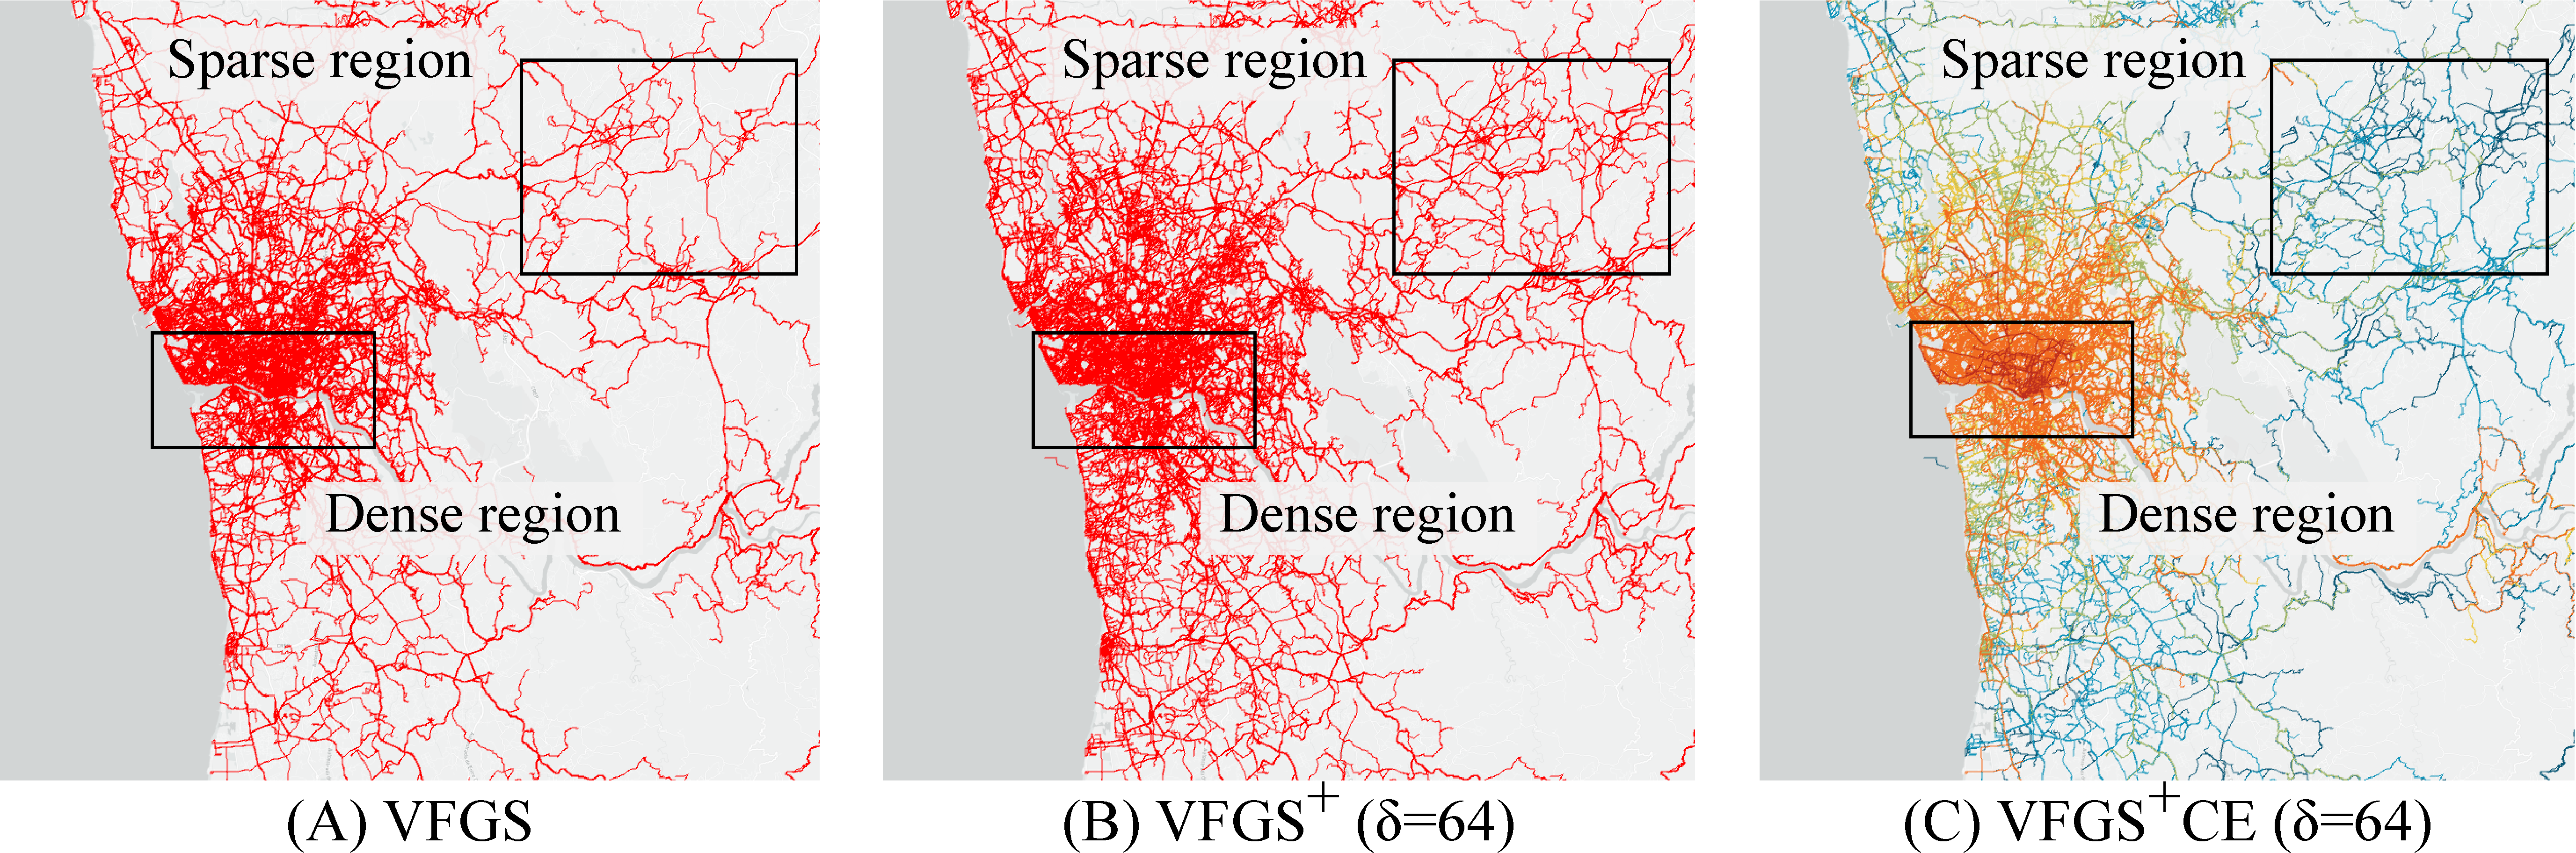
\includegraphics[width=0.48\textwidth]{pictures/problemsolveing/delta_motivation.pdf}
	\caption{The advanced approach $\avats$ on \pt{} ($\alpha = 0.5\%$).} 
	\label{fig:delta}
\end{figure}

%(see Algorithm~\ref{alg:plus})

Based on the two observations above, we can improve  $\vats$ by delivering richer information in the sparse regions and reducing visual clutter in the dense regions. $\avats$ in Algorithm~\ref{alg:plus} achieves both objectives using a perception tolerance parameter $\delta$, which models the perception capability of humans at the highest level of details.
Specifically, if pixel $(x,y)$ in canvas is covered by the result set $\oR$ at the highest level,
the pixels around $(x,y)$, i.e., from $(x-\delta, y-\delta)$ to $(x+\delta, y+\delta)$, does not need to be covered as  they are in the perception tolerance of human beings. We can easily modify $\vats$ in Algorithm~\ref{alg:greedy} to incorporate the perception tolerance parameter $\delta$ as shown in Algorithm~\ref{alg:plus}. $\avats$ measures the contribution of each trajectory $t_i$ w.r.t the augmented set $\oR^{+}$ in Line~\ref{line:deltamax},
where $\oR^{+}$ includes both the selected trajectories and their tolerance pixels (in Line~\ref{line:delta}).      

  
%Taking the above two observations into consideration, we can further improve the returning result of visual fidelity-guaranteed sampling approach $\vats$ by
%delivering rich information at sparse regions and reducing visual clutter in dense regions.
%In this section, we devise the advanced approach $\avats$ (see Algorithm~\ref{alg:plus}) to achieve the above two objectives.
%In specific, we introduce perception tolerance parameter $\delta$ in $\avats$, which models the perception capability of humans at the highest level of details.
%In other words, suppose the pixel $(x,y)$ in canvas is covered by the result set $\oR$ at the highest level,
%the pixels around $(x,y)$, i.e., from $(x-\delta, y-\delta)$ to $(x+\delta, y+\delta)$, are not necessary to cover because they are in the perception tolerance of human beings.


%It measures the contribution of each trajectory $t_i$ w.r.t the selected trajectory set $\oR$'s augmented set $\oR^{+}$, i.e., the selected trajectories and their tolerance pixels.
%.
%The augmented set $\oR^{+}$ will be updated by the selected trajectory $tmp$ and its tolerance pixels set (in Line~\ref{line:delta}).

%
\begin{algorithm}
    \caption{$\avats(\D,k=\alpha |\D|,\delta)$} \label{alg:plus}
    \begin{algorithmic}[1]
    \State Initialize result set $\oR \leftarrow \emptyset$
    \State Initialize augmented result set $\oR^{+} \leftarrow \emptyset$
    \While{$|\oR| < k$}
        \State $tmp \leftarrow argmax_{t_i \in \D} | t_i  \cup \oR^{+} |$ \label{line:deltamax}
        \State $\oR \leftarrow \oR \cup \{ tmp \}$
        \State $\oR^{+} \leftarrow \oR^{+} \cup \mathsf{augment}(tmp, \delta)$\label{line:delta}
    \EndWhile
    \For{each $t$ in $\D$} \Comment{Representative encoding} \label{line:s}
        \State $tr \leftarrow argmin_{t_i \in \oR}{|t-\mathsf{augment}(t_i, \delta)|}$
        \State $tr.\mathsf{cnt}++$ \label{line:e}
    \EndFor
    \State Return $\oR$
    \end{algorithmic}
\end{algorithm}


%Interestingly, the visual clutter large trajectory visualization problem can be further reduced
%by encoding representative trajectories in $\oR$ (the returning result of $\avats$) with colors.
%In particular, $\avats$ selects the trajectory with the largest uncovered pixels by taking the perception tolerance capability of humans into account at each iteration,
%instead of only choosing the trajectory with the largest uncovered pixels in $\vats$ (Algorithm~\ref{alg:greedy}).


$\vats$ in Algorithm~\ref{alg:greedy} selects trajectories with good representativeness and some trajectories will not be included into the result set $\oR$ even though they have more uncovered pixels w.r.t. $\oR$. The reason is that their uncovered pixels are too close to the pixels in the selected trajectories (i.e., within the tolerance area of selected pixels). Take Figure~\ref{fig:zoom}(A) for example, suppose $\delta=1$ and trajectory $a$ was selected at the first iteration, the trajectory to select in the second iteration is $c$ instead of $b$ because almost all pixels in $b$ is in the tolerance area of $a$'s. $\avats$ also provides excellent visual fidelity at arbitrary zooming resolutions. This is because it considers the perception tolerance parameter $\delta$  at the highest zoom level. For example, the zoom level in Figure~\ref{fig:zoom}(A) is higher than that in Figure~\ref{fig:zoom}(B).
According to our elaboration, $\avats$ selects trajectory $a$ and $c$ for Figure~\ref{fig:zoom}(A).
When the area is zoomed out, as shown in Figure~\ref{fig:zoom}(b), trajectory $a$ and $c$ still captures the main sketch of the underlying dataset (as gray cells shown).
We will further elaborate this phenomenon by the experimental study in Section~\ref{sec:exp}.



The visual clutter problem for large-scale trajectory visualization can be further alleviated by encoding the representativeness of the trajectories in $\oR$ with colors. We define the representativeness of a trajectory $t_i$ in $\oR$ as the number of trajectories in the dataset $\D$ that has $t_i$ as its nearest neighbor in $\oR$. The distance between trajectory $t$ and $t_i$ is defined as the number of pixels in $t$ that can not be covered by the augmented pixels of $t_i$. We compute the representativeness of each trajectory in $\oR$ from Line~\ref{line:s} to Line~\ref{line:e} in Algorithm~\ref{alg:plus}. Figure~\ref{fig:delta}(C) shows the visualization result by encoding trajectories with larger representativeness with warmer colors. There are more details in the sparse regions compared with the $\vats$ result in Figure~\ref{fig:delta}(A), and we can identify the main roads in the dense region with very warm colors.

%Thus, the selected trajectories in the dense region are more representative than those in sparse region.

\begin{figure}[t]
	\centering
	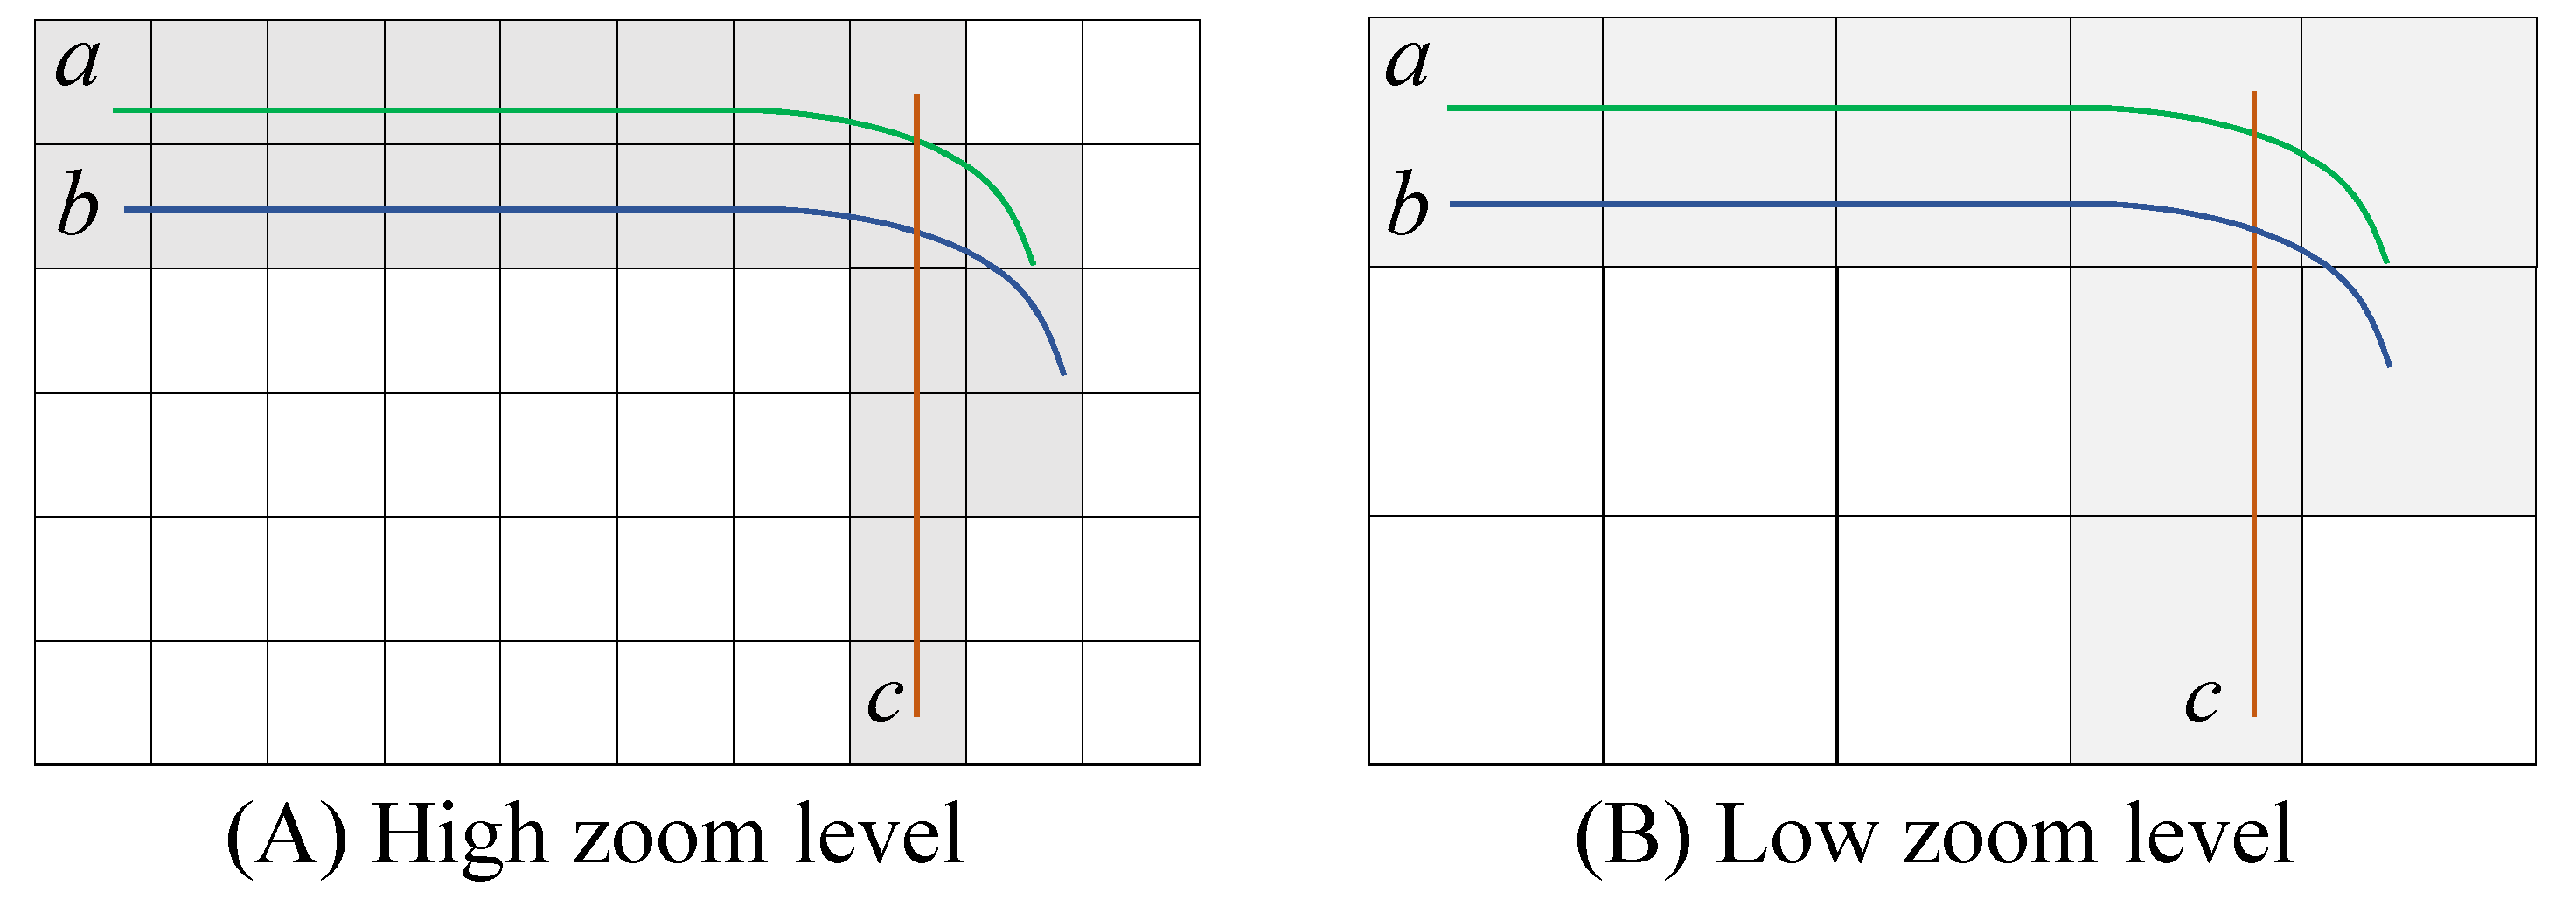
\includegraphics[width=0.45\textwidth]{pictures/problemsolveing/one_to_many.pdf}
	\vspace{-2mm}
	\caption{$\avats$ at different zoom levels.}	\label{fig:zoom} %An illustration of
    \vspace{-2mm}
\end{figure}






%(1) Richer Information Delivering: details aware; so Arbitrary zooming resolutions
%(2) Popularity Embedding: visual clutter



%\subsection{One-to-many strategy}~\label{sec:one_to_many}
%Since we detect the covered pixels in the highest level, two trajectories may be very close to each other but share very few pixels, which will lead to more information loss in the low zoom view as figure~\ref{fig:one_to_many}.
%We next elaborate a ``one-to-many'' strategy to further optimize the visual quality of our proposed technique.
%Recalling we use the highest zoom level to define the pixel size in the canvas.
%Thus, our visual quality guaranteed sampling algorithm is zoom-level oblivious, e.g., it guarantees the visual quality of result set $\oR$ at every zoom level.
%However, users always do not use/need the highest zoom level in visualization applications.
%For example, Google map shows city and streets at zoom level 1 and 15, respectively~\footnote{\url{https://developers.google.com/maps/documentation/}}.
%Motivated by the above observation, we devise ``one-to-many'' strategy by introducing a visual tolerance parameter $\delta$ to optimize the visual quality for users.
%Specifically, ,
%the ``one-to-many'' strategy will ignore all the pixels around $(x,y)$ within $\delta$ offset distance, i.e., all pixels from $(x-\delta, y-\delta)$ to $(x+\delta, y+\delta)$ will be skipped.
%We will demonstrate the effectiveness of the visual tolerance $\delta$ in experimental evaluations.
%
%%https://developers.google.com/maps/documentation/maps-static/dev-guide#Zoomlevels
%\begin{figure}[t]
%	\centering
%	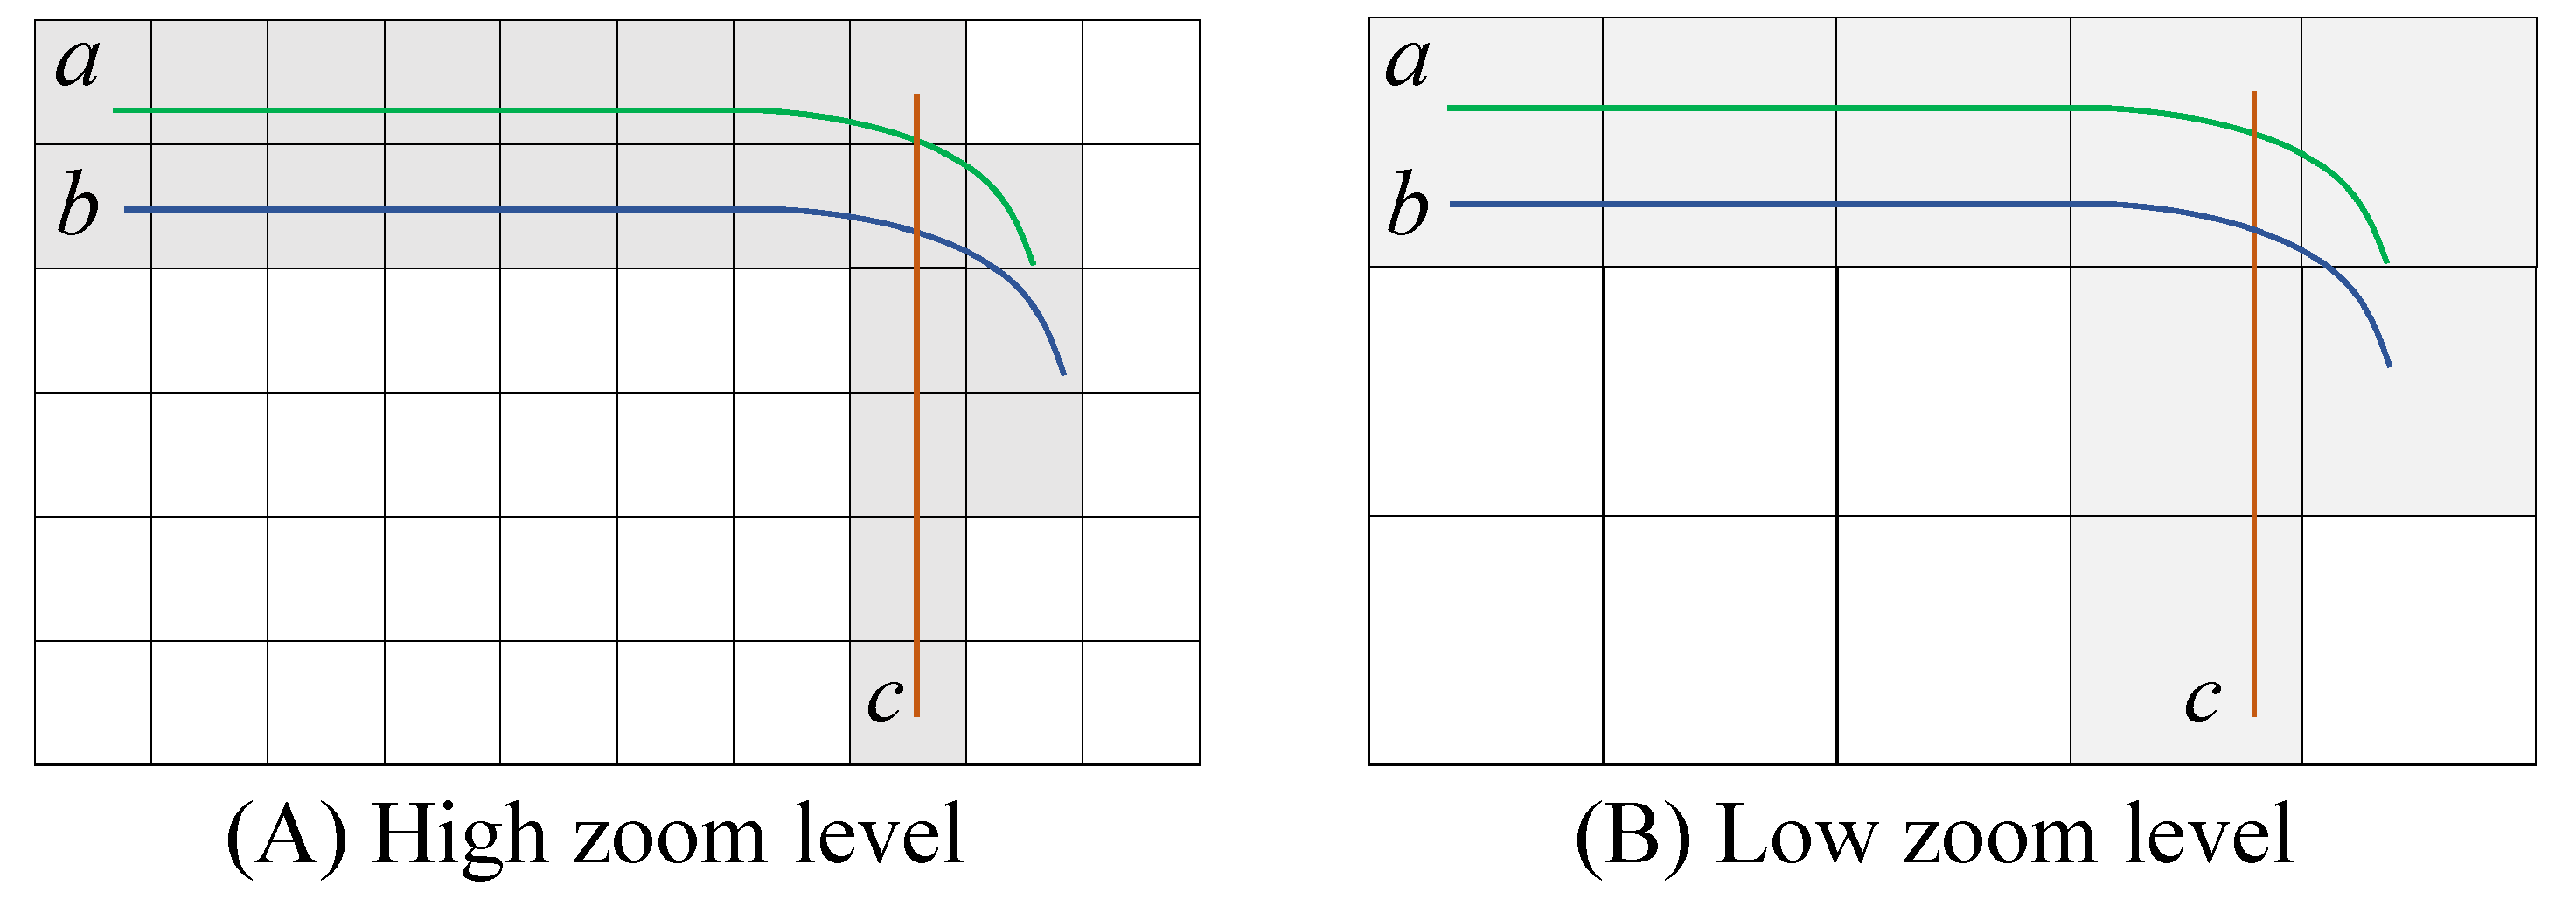
\includegraphics[width=0.4\textwidth]{pictures/problemsolveing/one_to_many.pdf}
%	\vspace{-5mm}
%	\caption{Resolution inconsistency}
%	\vspace{-5mm}
%	\label{fig:one_to_many}
%\end{figure}


%Specifically, $\avats$ incorporates a parameter $\delta$ during trajectory selection process in $\vats$ .
%In particular, we employ the parameter $\delta$ to model the end user's perception ability at the most high level of details.
%Surprisingly, our advance approach $\avats$ not only provides better visualization result when comparing with $\vats$ with the same sampling rate
%(e.g., Figure~\ref{fig:delta}(a) and (b) are the returning result of $\vats$ and $\avats$ respectively),
%but also embeds the popularity of selected trajectories by encoding the rest trajectories in the dataset in them,
%e.g., Figure~\ref{fig:delta}(c) is the visual result of $\avats$ with color encoded popularity.



